\documentclass{beamer}

\usepackage{ucs}
\usepackage[utf8x]{inputenc}
\usepackage[english,russian]{babel}
%\usepackage{times}

\usepackage{color, colortbl}
\usepackage{rotating} 
\usepackage{graphicx}
\usepackage{algorithmic}
\usepackage{verbatim}
\usepackage{movie15}
\usepackage{media9}
\usepackage{xcolor}

\usetheme{PetrSU-CS}

%%%%
% Преамбула: основные параметры презентации
% Отредактируйте в соответствии с комментариями
%

\title[%
    % Краткое название работы не используется в этой презентации!
    Веб-сервис измерения активности аудитории сетевых СМИ
]{%
    % Полное название работы отображается на титульной странице
    % Разработка веб-сервиса измерения активности аудитории сетевых СМИ на основе портала <<Российская общественная инициатива>>
    Разработка программной системы для проявления, регистрации и анализа гражданской активности посетителей веб-сайтов
}

% Подзаголовком опишите тип работы:
% - Курсовая работа
% - Выпускная квалификационная работа бакалавра
% - Дипломная работа
% - Магистерская диссертация
\subtitle{Выпускная квалификационная работа бакалавра\\
Направление 010400 --- Прикладная математика и информатика}

\author[%
    % Имя и фамилия автора работы отображаются на каждом слайде в нижнем колонтитуле
    Александр Шварц
]{%
    % Имя, отчество и фамилия автора работы отображаются на титульном слайде
    Александр Евгеньевич Шварц
}

\date[%
    % Дата защиты
    22.04.2015
]{%
    % Руководитель
    Научный руководитель: к.ф.-м.н.,~А.~С.~Румянцев
}

\institute[%
    % Краткое название организации не используется в этой презентации
    ПетрГУ
]{%
    % Полное название организации и подразделения
    Петрозаводский государственный университет\\
	Математический факультет\\
    Кафедра прикладной математики и кибернетики
}


%%%%
%
% Начало содержимого слайдов
%

\begin{document}

\begin{frame}
  \titlepage
\end{frame}


\begin{frame}
\frametitle{Активное гражданское общество}
\begin{block}{Гражданское общество}
Совокупность граждан государства, а также комплекс самоорганизующихся и самоуправляемых общественных институтов, реализующих частные права и свободы этих граждан и, как правило, юридически регламентирующиеся со стороны государства
\end{block}

\begin{block}{Гражданская активность}
деятельное, мотивированное участие индивидов в преобразовании объективных социальных условий, в таком их изменении, которое способствует более полному достижению интересов и удовлетворению потребностей.
\end{block}
\end{frame}

\section{Методы измерения активности}
\begin{frame}
\frametitle{Электронно-цифровое общество}

\begin{block}{Электронно-цифровое общество}
Общество, представители которого используют электронные технологии для хранения, распространения и обработки информации и данных. 
\end{block}

Цели использования сети интернет:
\begin{enumerate}
  \item поиск информации;
  \item общение;
  \item слежение за последними новостями.
\end{enumerate}

\end{frame}

\begin{frame}
\frametitle{Способы проявления гражданской активности в сети интернет}
\begin{itemize}
  \item открытые обращения (youtube, блоги); \vspace{0.5cm}
  \item онлайн-голосование, петиции.
\end{itemize}

Платформы для публикации инициатив:
\begin{enumerate}
  \item 
  \textcolor{green}{\large Российская общественная инициатива} (\url{www.roi.ru});
    \begin{itemize}
    \item[$+$] создан по указу Президента;
    \item[$+$] рассмотрение экспертной группой;
    \item[$+$] один человек -- один голос.
    \end{itemize}
  \item Глобальная платформа для ваших кампаний (\url{www.change.org});
  \item Платформа для петиций РуНета (\url{www.onlinepetition.ru});
  \item Наше мнение (\url{www.mypetition.ru}).
\end{enumerate}
\end{frame}

\section{Цель работы}
\begin{frame}
\frametitle{Цель работы}
\begin{block}{Цели}
\begin{enumerate}
  \item Разработать программную систему для проявления, регистрации и анализа гражданской активности аудитории веб-сайтов.
\end{enumerate}
\end{block}
Задачи:
\begin{itemize}
  \item предложить метод реализации и регистрации активности аудитории веб-сайтов;
  \item разработать архитектуру системы;
  \item разработать модуль работы с посетителями веб-сайтов;
  \item разработать модуль анализа данных.
\end{itemize}
\end{frame}

\section{Метод измерения активности}
\begin{frame}
\frametitle{Метод реализации и регистрации активности аудитории веб-сайтов}
Веб-сайты предоставят своим посетителям возможность проявить гражданскую активность на портале РОИ.

\textcolor{lightgray}{По сути веб-сайты будут <<рекламировать>> актуальные инициативы с портала.}

\vspace{0.5cm}
Метод заключается в:
\begin{itemize}
  \item отображении на веб сайте с помощью специального приложения информации об актуальных инициативах c портала РОИ;
  \item регистрации переходов по инициативам в базе данных с помощью отправки параллельного POST запроса.
\end{itemize}

\end{frame}

\begin{frame}
\frametitle{Сетевые Издания}
\begin{block}{Сетевое издание}
Сайт в сети Интернет, зарегистрированный в качестве СМИ.
\end{block}
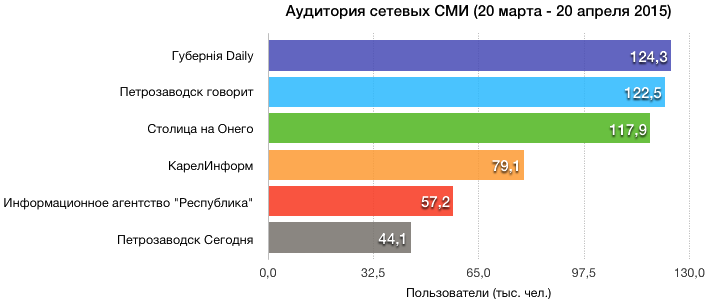
\includegraphics[width=0.84\textwidth]{images/usersSMI}

Особенности сетевых изданий:
\begin{itemize}
  \item характер статей побуждает к действиям;
  \item большая аудитория.
\end{itemize}
\end{frame}

\section{Архитектура системы}
\begin{frame}
\frametitle{Архитектура системы}
Запись переходов по инициативам

\vspace{0.5cm}
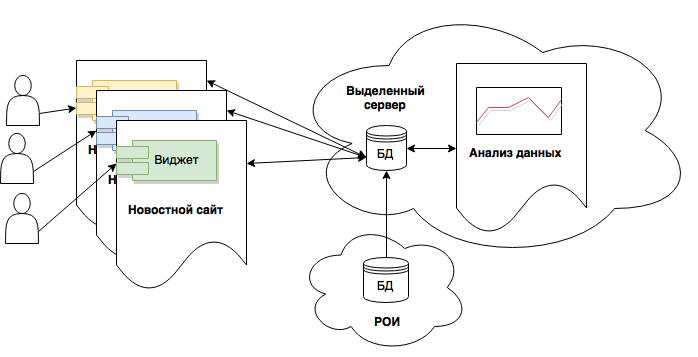
\includegraphics[width=1\textwidth]{images/arch2}
\end{frame}

\section{Модуль работы с посетителями СМИ}
\begin{frame}
\frametitle{Модуль работы с посетителями веб-сайтов}
\begin{columns}[T]
\begin{column}{0.55\textwidth}
Модуль работы с посетителями веб-сайтов выполнен в форме легко конфигурируемого виджета.

\vspace{0.5cm}
Конфигурируемые параметры:
\begin{itemize}
  \item тема (внешний вид);
  \item регионы, к которым относятся инициативы;
  \item количество отображаемых записей (для каждого блока).
\end{itemize}
\end{column}
\begin{column}{0.45\textwidth}
\vspace{0.5cm}
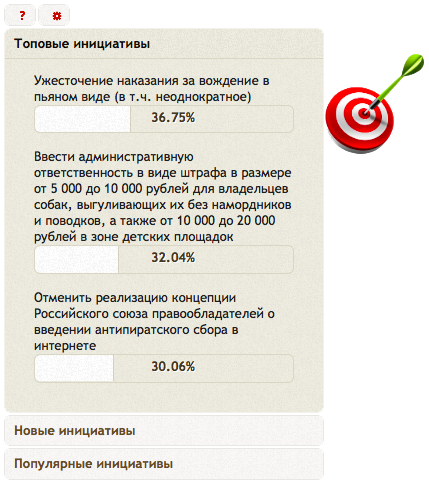
\includegraphics[width=1.0\textwidth]{images/widget}
\end{column}
\end{columns}
\end{frame}

\section{Модуль для анализа данных}

\begin{frame}
\frametitle{Модуль анализа данных}
\vspace{0.5cm}
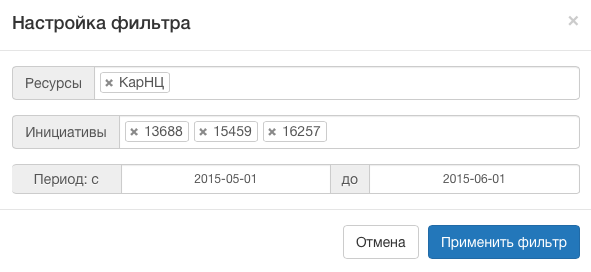
\includegraphics[width=0.7\textwidth]{images/filter}

Фильтр содержит следующие критерии:
\begin{enumerate}
  \item названия ресурсов --- $r \in R$;
  \item даты активности (период) --- $[d_{from}, d_{to}], d_{from}, d_{to} \in D$;
  \item номера инициатив --- $i \in I$.
\end{enumerate}
\end{frame}

\begin{frame}
\frametitle{Модуль анализа данных}
\begin{columns}[T]
\begin{column}{0.30\textwidth}
Модуль анализа позволяет построить графики и таблицы по заданному фильтру.

\vspace{1.5cm}

Рейтинг ресурсов:
\begin{tabular}{|l|l|}
\hline
Имя ресурса & Переходы\\
\hline
сайт 1 & $n_1$\\
\hline
\dots & \\
\hline
сайт i & $n_i$\\
\hline
\dots & \\
\hline
сайт $N$ & $n_{N}$\\
\hline
\end{tabular}
\end{column}
\begin{column}{0.70\textwidth}
\vspace{0.2cm}
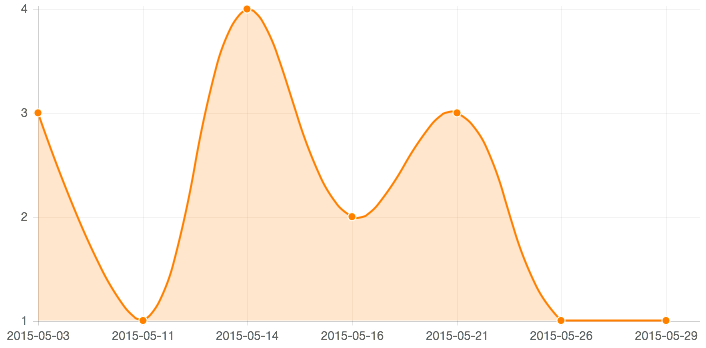
\includegraphics[width=0.95\textwidth]{images/chart}

\hspace{1cm} $n_i$ --- количество переходов с сайта $i$

\hspace{1cm} $n_1 \geq n_i \geq n_{N}$


\hspace{1cm} По оси абсцисс отмечаются $d \in D$

\hspace{1cm} По оси ординат отмечаются $\sum\limits_{i \in I, r \in R} x (r,i,d)$

\end{column}
\end{columns}
\end{frame}


\begin{frame}
\frametitle{Результаты}
\begin{itemize}
  \item[$+$] предложен метод измерения гражданской активности аудитории веб-сайтов;
  \item[$+$] разработана архитектура системы;
  \item[$+$] разработан модуль работы с посетителями веб-сайтов в форме виджета;
  \item[$+$] разработан модуль анализа данных в форме веб-сервиса;
  \item[$+$] проведено тестирование.
\end{itemize}

\begin{center}\bf\LARGE
Спасибо за внимание!
\end{center}

\end{frame}


\end{document}